\documentclass[12pt, a4paper]{article}
\usepackage[top=1.0in, bottom=1.0in, left=0.8in, right=0.8in]{geometry}

\setlength{\parskip}{\baselineskip}%
\setlength{\parindent}{0pt}%
\usepackage{bookmark}
\usepackage[]{graphicx}
\usepackage{enumitem}
\usepackage{amsmath}
\usepackage{relsize}
\usepackage{cprotect}
\usepackage{amsmath, amsfonts}
\usepackage{siunitx}
\usepackage{mathrsfs}
\usepackage{framed}
\usepackage{enumitem}
\usepackage{tikz}
\usepackage{circuitikz}
\usepackage{float}
\usepackage[english]{babel}
\usepackage{blindtext}
\usepackage{listings}
\usepackage{algpseudocode}

\newlist{notes}{enumerate}{1}
\setlist[notes]{label=\textbf{Note:} ,leftmargin=*}

\newlist{hints}{enumerate}{1}
\setlist[hints]{label=\textbf{Hint:} ,leftmargin=*}

\usepackage{xcolor}
\usepackage{color}
\definecolor{com1}{RGB}{125,125,125}
\definecolor{comment}{RGB}{140,115,115}
\definecolor{numbering}{rgb}{0.2,0.2,0.2}
\definecolor{key}{RGB}{0,0,180}
\definecolor{in}{RGB}{0,100,0}
\definecolor{out}{RGB}{100,30,30}
\definecolor{bg}{RGB}{245,245,245}
\definecolor{bgLight}{RGB}{250,250,250}
\definecolor{string}{RGB}{0,150,0}

\usepackage{hyperref}
\hypersetup{
    colorlinks=true,
    linkcolor=blue,
    filecolor=magenta,      
    urlcolor=blue,
}
\urlstyle{same}

\usepackage{listings}

\lstdefinestyle{py_code}{ %
    backgroundcolor=\color{bg},      % choose the background
    basicstyle=\ttfamily\small,		      % fonts
    breakatwhitespace=false,         % automatic breaks at whitespace ?
    breaklines=true,                 % sets automatic line breaking
    captionpos=b,                    % caption-position - bottom
    commentstyle=\itshape\color{comment},    % comment style
    extendedchars=true,              % use non-ASCII
    frame=single,	                   % single frame around the code
    keepspaces=true,                 % keeps spaces in text
    keywordstyle=\bfseries\color{key},% keyword style
    language=Python,                 	  % the language of the code
    morekeywords={Null},       % add more keywords to the set
    numbers=left,                    % line_numbers (none, left, right)
    numbersep=10pt,                  % line_no - code dist
    numberstyle=\footnotesize\color{numbering}, % line_no style
    rulecolor=\color{black},         % frame_color [!always set]
    showspaces=false,                % show spaces everywhere
    showstringspaces=false,          % 
    showtabs=false,                  % 
    stepnumber=1,                    % step b/w two line-no
    stringstyle=\color{string},     % string literal style
    tabsize=2,	                       % sets default tabsize to 2 spaces
    title=\lstname,                  % show the filename
    escapeinside={(*}{*)},			  % escape from style inside (* *)
    xleftmargin=\parindent,
    belowskip=-1.3 \baselineskip,
    aboveskip=1.0 \baselineskip,
    columns=fullflexible,
    xleftmargin=0.15in,
}
\lstnewenvironment{py_code}
{\lstset{style=py_code}}
{}

\lstdefinestyle{psudo}{ %
    backgroundcolor=\color{bgLight},   % choose the background
    basicstyle=\ttfamily\small,		      % fonts
    breakatwhitespace=false,         % automatic breaks at whitespace ?
    breaklines=true,                 % sets automatic line breaking
    captionpos=b,                    % caption-position - bottom
    commentstyle=\itshape\color{com1},          % comment style
    extendedchars=true,              % use non-ASCII
    keepspaces=true,                 % keeps spaces in text
    language=C,                 	  % the language of the code
    morekeywords={type,NULL, True, False},       % add more keywords to the set
    showspaces=false,                % show spaces everywhere
    showstringspaces=false,          % 
    showtabs=false,                  % 
    tabsize=2,	                       % sets default tabsize to 2 spaces
    title=\lstname,                  % show the filename
    escapeinside={(*}{*)},			  % escape from style inside (* *)
    belowskip=-1.8 \baselineskip,
    aboveskip=0.9 \baselineskip,
    columns=fullflexible,
    xleftmargin=0.2in,
    frame=tb,
    framexleftmargin=16pt,
    framextopmargin=6pt,
    framexbottommargin=6pt, 
    framerule=0pt,
}

\lstnewenvironment{psudo}
{\lstset{style=psudo}}
{}

\graphicspath{ ./ }

\title{\textbf{EE2703 : Applied Programming Lab \\  \vspace*{1cm} End Semester Exam \\ \vspace*{1cm} Antenna Currents in a Half-Wave Dipole Antenna}} 
\author{Chagari Koushal Kumar Reddy \\ EE20B023} % Author name

\date{\today} % Date for the report

\begin{document}		

\maketitle % Insert the title, author and date
\clearpage

\tableofcontents
\clearpage

\section{Problem Statement}
There is a long wire carrying current $I(z)$ in a dipole antenna of half length $50$cm. The standard analysis of dipole antennas assumes that the current distribution is given by:
\begin{equation*}
    I(z) =    \left\{
        \begin{array}{ll}
              Im\sin(k(l-z)) \qquad      \   0 \le z \le l \vspace*{0.4cm} \\ 
              Im\sin(k(l+z)) \qquad       -l \le z < 0  
        \end{array} 
        \right. 
\end{equation*}
This assumed value of current is generally used to find the radiation field. We want to know whether this was a good assumption by calculating the actual values of the current in the dipole. We finally plot these 2 graphs in the same plot and compare them.

% \section{Method of Approach}
% The half dipole length is assumed to be $l = 0.5$m (Quarter Wavelength). The dipole is then divided into sections each of length 
% $dz$. We then initialize the points along the dipole length and the currents there as vectors $z$ and $I$. There are some very important \textbf{boundary conditions} to be followed:
% \begin{itemize}
%     \item The current at either ends of the dipole is 0. This means $I[0] = I[2N] = 0$ 
%     \item The current at $z = 0$ is determined by the circuit driving it and is taken as $I_{m}$. This means $I[N] = I_{m}$ 
% \end{itemize}
% We know from Ampere's law that for $H_{\phi}(z,r=a)$:
% \begin{equation*}
%     2\pi aH_{\phi}(z_{i}) = I_{i}
% \end{equation*}
% This can be written as a matrix equation as shown below:
% \begin{equation*}
%     \begin{pmatrix}
%         H_{\phi}[z_{1}]  \\
%         \ldots \\
%         H_{\phi}[z_{N-1}]  \\
%         H_{\phi}[z_{N+1}]  \\
%         \ldots \\
%         H_{\phi}[z_{2N-1}]  \\
%     \end{pmatrix} = \frac{1}{2 \pi a}
%     \begin{pmatrix}
%         1 \; \ldots \quad 0 \quad 0 \; \ldots \quad 0 \\
%         \ldots \ldots \ldots \ldots \ldots \ldots \\
%         0 \; \ldots \quad 1 \quad 0 \; \ldots \quad 0 \\
%         0 \; \ldots \quad 0 \quad 1 \; \ldots \quad 0 \\
%         \ldots \ldots \ldots \ldots \ldots \ldots \\
%         0 \; \ldots \quad 0 \quad 0 \; \ldots \quad 1 \\
%     \end{pmatrix}
%     \begin{pmatrix}
%         J_{1} \\
%         \ldots \\
%         J_{N-1} \\
%         J_{N+1} \\
%         \ldots \\
%         J_{2N-1}
%     \end{pmatrix}
% \end{equation*}
% Here note that vector $J$ is the vector of unknown currents. Hence it's dimensions are $2N-2$ by $2N-2$.


% The second method to calculate $H_{\phi}(z,r=a)$ involves calculation of the magnetic vector potential $\vec{A}(r,z)$:
% \begin{equation*}
%     A_{z,i} = \frac{\mu_{o}}{4\pi}\sum _{j}{} \frac{I_{j}exp(-jkR_{ij})dz_{j}}{R_{ij}}
% \end{equation*}
\section{Pseudocodes, Codes and Plots}
\subsection{Section 1}
\subsubsection{Pseudocode}

\begin{enumerate}

  \item \quad INIT All required constants (c,$\mu_{o},l,dz,\lambda,k$)
  \item \quad INIT Location of known, unknown currents ($z$, $u$)
  \item \quad INIT Vector contaning all currents, unknown currents ($I$, $J$)
  \item \quad INIT Boundary conditions of $I$ ($I[0]=I[2N]=0$, $I[N]=I_{m}$)
\end{enumerate}

\subsubsection{Code}
\vspace*{0.4cm}
\hrule
    \begin{lstlisting}[language=Python]
    i = p.linspace(-N,N,2*N+1)
    z = i*dz
    I = p.zeros((2*N+1),dtype = complex)
    I[0] = 0 ; I [2*N] = 0 ; I[N] = Im
    
    # 2N - 2 locations of unknown currents
    # Deleting the first, middle and last entries
    u = p.delete(z,(0,N,2*N))           
    J = p.zeros(2*N-2)
    \end{lstlisting}
\hrule
\subsubsection{Explanation}
The locations at which we compute the currents are given by $z$. $z$ has $2N+1$ elements varying from $-l$ to $l$.
The $2N+1$ currents are stored in the $I$ vector. Since we know the values of $I$ at $0,N,2N$ there are $2N-2$ unknown currents. The corresponding unknown current densities are stored in $J$. The corresponding unknown current locations are also computed and stored in the vector $u$.
\subsubsection{Output Vectors (For $N=4$)}
    \begin{itemize}
        \item   $z : \begin{bmatrix} -0.5 &  -0.375 & -0.25 & -0.125 & 0. & 0.125 & 0.25 & 0.375 & 0.5 \end{bmatrix} $
        \item   $u :  \begin{bmatrix} -0.375 & -0.25 &  -0.125 &  0.125 &  0.25 &  0.375 \end{bmatrix}$
        \item   $I :  \begin{bmatrix} 0. & 0. & 0. & 0. & 1. & 0. & 0. & 0. & 0.\end{bmatrix}$
        \item   $J :  \begin{bmatrix} 0. & 0. & 0. & 0. & 0. & 0. \end{bmatrix}$
    \end{itemize}
\subsection{Section 2}
\subsubsection{Pseudocode}
\begin{enumerate}

    \item \quad FUNCTION: M
    \item \quad \quad INPUT: Number of sections in each half of antenna $N$
    \item \quad \quad CALCULATE Matrix $M$ using identity matrix and radius of wire $a$
    \item \quad \quad RETURN Matrix $M$
    \item \quad ENDFUNCTION
  \end{enumerate}
\subsubsection{Code}
\vspace*{0.4cm}
\hrule
    \begin{lstlisting}[language=Python]
    def M(n):
    # Matrix M of order 2*N-2 by 2*N-2
        return (1/(2*pi*a))*p.identity(2*n-2)
    \end{lstlisting}
\hrule
\subsubsection{Explanation}
In the first method to calculate $H_{\phi}(z,r=a)$, as explained above a matrix M needs to be created. This function generates such a matrix $M$ taking input as $N$. Here $a$ is the radius of the wire.
\vspace*{0.4cm}
\begin{equation*}
    M = \frac{1}{2\pi a}
    \begin{pmatrix}
        1 \; \ldots \quad 0 \quad 0 \; \ldots \quad 0 \\
        \ldots \ldots \ldots \ldots \ldots \ldots \\
        0 \; \ldots \quad 1 \quad 0 \; \ldots \quad 0 \\
        0 \; \ldots \quad 0 \quad 1 \; \ldots \quad 0 \\
        \ldots \ldots \ldots \ldots \ldots \ldots \\
        0 \; \ldots \quad 0 \quad 0 \; \ldots \quad 1 \\
    \end{pmatrix}
\end{equation*}
\subsubsection{Output Vectors (For $N=4$)}
\begin{itemize}
    \item
    $ M = 
    \begin{bmatrix}
    15.92  &  0  &   0  &  0  &   0  &  0   \\
    0   & 15.92  & 0  &  0 &  0  &  0  \\
    0   & 0  & 15.92  &  0 &  0  &  0  \\
    0   & 0  & 0  &  15.92 &  0  &  0  \\
    0   & 0  & 0  &  0 &  15.92  &  0  \\
    0   & 0  & 0  &  0 &  0  &  15.92  \\
    \end{bmatrix}
    $
\end{itemize}
\subsection{Section 3}
\subsubsection{Pseudocode}
\begin{enumerate}

    \item \quad CALCULATE Distances for all pairs of $z_{i},z_{j}$ for $i,j$ from $0$ to $2N$ ($R_{z}$)
    \item \quad CALCULATE Distances for unknown currents by removing $z = 0, N, 2N$ ($R_{u}$)
    \item \quad CALCULATE Contribution to vector potential by unknown current sources ($P$)
    \item \quad CALCULATE Contribution to vector potential by current $I_{N}$ ($P_{B}$) 
  \end{enumerate}
\subsubsection{Code}
\hrule
    \begin{lstlisting}[language=Python]
    # Meshgrid generates 2D matrices which are used to find the 
    # distance between 2 points zi, zj as i,j go from 0 to 2N+1
    
    zj,zi = p.meshgrid(z,z)
    zij = p.zeros((2*N+1,2*N+1))
    zij = (zi - zj)**2
    Rz = p.zeros((2*N+1,2*N+1))
    # Since radius of the wire, a = r
    Rz = p.sqrt(a**2 + zij)               
    print("Rz : ", (Rz).round(2))
    
    # Here we are calculating distances for unknown current locations
    
    zj,zi = p.meshgrid(u,u)
    zij = p.zeros((2*N-2,2*N-2))
    zij = (zi - zj)**2
    Ru = p.zeros((2*N-2,2*N-2))
    # Since radius of the wire, a = r
    Ru = p.sqrt(a**2 + zij)               
    print("Ru : ", (Ru).round(2))
    
    # Calculation of matrices P and Pb
    
    j = complex(0,1)         # Defining j       
    P = p.zeros((2*N-2,2*N-2), dtype = complex)
    P = mu0*p.exp(-j*k*Ru)*dz/(4*pi*Ru)
    print("P*1e8 : ", (P*1e8).round(2))
    
    Pb = p.zeros((2*N-2),dtype = complex)
    # From Rz[:N], we don't need distances to z = 0, z = N, z = 2N
    Rz_del = p.delete(Rz[:,N],(0,N,2*N))
    Pb = mu0*p.exp(-j*k*Rz_del)*dz/(4*pi*Rz_del)
    print("Pb*1e8 : ", (Pb*1e8).round(2))
    \end{lstlisting}
\hrule
\subsubsection{Explanation}
$R_{ij}$ is the distance of the point $\vec{r} + z_{i}\hat{z}$ and the source $z_{j}\hat{z}$. So $R_{ij}$ value is calculated as:
\begin{equation*}
    R_{ij} = a^{2} + (z_{i}-z_{j})^{2}
\end{equation*}
Another name for the above is $R_{z}$. Similarly we create $R_{u}$ which is a vector of distances of unknown currents. We also compute the matrix $P$ which is given by:
\begin{equation*}
    P_{ij} = \frac{\mu_{o}}{4\pi}\frac{exp(-jkR_{ij})}{R_{ij}}dz
\end{equation*}
$P_{B}$ is the vector corresponding to the contribution to the vector potential due to current $I_{N}$ and is given by:
\vspace*{0.3cm}
\begin{equation*}
    P_{B} = \frac{\mu_{o}}{4\pi}\frac{exp(-jkR_{iN})}{R_{iN}}dz
\end{equation*}
\subsubsection{Output Vectors (For $N=4$)}
\begin{itemize}
    \item $ R_{z} : 
    \begin{bmatrix}
    0.01  &  0.13  &   0.25  &  0.38  &   0.5  &  0.63 & 0.75 & 0.88 & 1  \\
    0.13  &  0.01  &   0.13  &  0.25  &   0.38  &   0.5  &  0.63 & 0.75 & 0.88  \\
    0.25  &  0.13  &   0.01  &  0.13  &   0.25  &  0.38 & 0.5 & 0.63 & 0.75  \\
    0.38  &  0.25  &   0.13  &  0.01  &   0.13  &  0.25 & 0.38 & 0.5 & 0.63  \\
    0.5  &  0.38  &   0.25  &  0.13  &   0.01  &  0.13 & 0.25 & 0.38 & 0.5  \\
    0.63  &  0.5  &   0.38  &  0.25  &   0.13  &  0.01 & 0.13 & 0.25 & 0.38  \\
    0.75  &  0.63  &   0.5  &  0.38  &   0.25  &  0.13 & 0.01 & 0.13 & 0.25  \\
    0.88  &  0.75  &   0.63  &  0.5  &   0.38  &  0.25 & 0.13 & 0.01 & 0.13  \\
    1  &  0.88  &   0.75  &  0.63  &   0.5  &  0.38 & 0.25 & 0.13 & 0.01  \\
    \end{bmatrix} $
    \item $R_{u} : 
    \begin{bmatrix}
    0.01 & 0.13 & 0.25 & 0.5 & 0.63 & 0.75 \\
    0.13 & 0.01 & 0.13 & 0.38 & 0.5 & 0.63 \\
    0.25 & 0.13 & 0.01 & 0.25 & 0.38 & 0.5 \\
    0.5 & 0.38 & 0.25 & 0.01 & 0.13 & 0.25 \\
    0.63 & 0.5 & 0.38 & 0.13 & 0.01 & 0.13 \\
    0.75 & 0.63 & 0.5 & 0.25 & 0.13 & 0.01 \\
    \end{bmatrix}$
    \item $P*1e8 : 
    \\
    \\
    \hspace*{-1cm}
    \begin{bmatrix}
    124.94-3.93j &  9.2 -3.83j &  3.53-3.53j &  -0. -2.5j   & -0.77-1.85j & -1.18-1.18j \\
    9.2 -3.83j & 124.94-3.93j &  9.2 -3.83j  &  1.27-3.08j &  -0.-2.5j & -0.77-1.85j \\
    3.53-3.53j &   9.2 -3.83j & 124.94-3.93j &  3.53-3.53j &  1.27-3.08j & -0.-2.5j \\
    -0.  -2.5j &   1.27-3.08j &  3.53-3.53j & 124.94-3.93j &  9.2 -3.83j & 3.53-3.53j \\
    -0.77-1.85j &  -0.  -2.5j  &  1.27-3.08j &  9.2 -3.83j & 124.94-3.93j & 9.2 -3.83j \\
    -1.18-1.18j &  -0.77-1.85j &  -0.  -2.5j  &  3.53-3.53j &  9.2 -3.83j & 124.94-3.93j \\
    \end{bmatrix}
    $
    \item $ P_{B}*1e8 : 
    \begin{bmatrix}
        1.27-3.08j & 3.53-3.53j & 9.2 -3.83j & 9.2 -3.83j & 3.53-3.53j & 1.27-3.08j
    \end{bmatrix}
    $
\end{itemize}
\subsection{Section 4}
\subsubsection{Pseudocode}
\begin{enumerate}
    \item \quad CALCULATE Contribution to Magnetic field density by unknown current sources ($Q$)
    \item \quad CALCULATE Contribution to Magnetic field density by current $I_{N}$ ($Q_{B}$) 
  \end{enumerate}
\subsubsection{Code}
\hrule
    \begin{lstlisting}[language=Python]
        # Q corresponds to contribution of unknown currents to H
        Q = p.zeros((2*N-2,2*N-2),dtype = complex)
        Q[:] = P[:]*a*(1/mu0)*((j*k/Ru[:]) + (1/(Ru[:]**2)))
        print("Q : ",(Q).round(2))
        
        # Qb corresponds to contribution of In to H
        Qb = p.zeros((2*N-2,1), dtype = complex)
        Qb[:,0] = Pb[:]*a*(1/mu0)*((j*k/Rz_del) + 1/(Rz_del**2))
        print("Qb : ", (Qb).round(2))
    \end{lstlisting}
\hrule
\subsubsection{Explanation}
$Q$ denotes the contribution of the unknown currents to Magnetic field density $H$. It is given by:
\begin{equation*}
    Q_{ij} = P_{ij} \frac{r}{\mu_{o}}(\frac{jk}{R_{ij}} + \frac{1}{R_{ij}^{2}})
\end{equation*}
$Q_{B}$ denotes the contribution of $I_{N}$ to the Magnetic field density. It is given by:
\begin{equation*}
    Q_{B} = P_{B} \frac{r}{\mu_{o}}(\frac{jk}{R_{iN}} + \frac{1}{R_{iN}^{2}})
\end{equation*}
\subsubsection{Output Vectors (For $N=4$)}
\begin{itemize}
    \item $
    Q $: \\ \\
    \hspace*{-1cm}
    \footnotesize
    $
    \begin{bmatrix}
    (99.521-0.001j) & (0.054-0.001j) & (0.008-0.001j) & (0.001-0.001j) & (0.001-0.001j) & -0.001j\\
    (0.054-0.001j) & (99.521-0.001j) & (0.054-0.001j) & (0.003-0.001j) & (0.001-0.001j) & (0.001-0.001j)\\
    (0.008-0.001j) & (0.054-0.001j) & (99.521-0.001j) & (0.008-0.001j) & (0.003-0.001j) & (0.001-0.001j)\\
    (0.001-0.001j) & (0.003-0.001j) & (0.008-0.001j) & (99.521-0.001j) & (0.054-0.001j) & (0.008-0.001j)\\
    (0.001-0.001j) & (0.001-0.001j) & (0.003-0.001j) & (0.054-0.001j) & (99.521-0.001j) & (0.054-0.001j)\\
    -0.001j & (0.001-0.001j) & (0.001-0.001j) & (0.008-0.001j) & (0.054-0.001j) & (99.521-0.001j)\\
    \end{bmatrix}
    $
    \normalsize
    \item $
    Q_{B} :$
    \footnotesize
    $\begin{bmatrix}
        (0.003-0.001j) \\ (0.008-0.001j) \\ (0.054-0.001j) \\ (0.054-0.001j) \\ (0.008-0.001j) \\ (0.003-0.001j)\\
        \end{bmatrix}
    $
    \normalsize
\end{itemize}
\subsection{Section 5}
\subsubsection{Pseudocode}
\begin{enumerate}
    \item \quad CALCULATE Current Density according to final equation by taking inverse ($\vec{J}$)
    \item \quad CALCULATE Current from $\vec{J}$ and boundary conditions ($I$)
    \item \quad CALCULATE Assumed value of current in dipole antenna ($I\_assumed$)
    \item \quad PLOT Current vs $z$ for $N=4$ and $N=100$ 
  \end{enumerate}
\subsubsection{Code}
\hrule
    \begin{lstlisting}[language=Python]
        J = p.dot(p.inv(M(N)-Q),Qb)*Im
        print("J : ", J)

        # Finding current vector with boundary conditions
        I[1:N] = J[:N-1,0]
        I[N+1:-1] = J[N-1:,0]
        print("I : ", I)

        # Finding assumed current in the dipole antenna

        I_assumed = p.zeros((2*N+1))
        I_assumed[:] = Im*p.sin(k*(l-z[:]))

        p.figure(1)
        p.grid(True)
        p.plot(z,abs(I), label = 'Actual Current')
        p.plot(z,abs(I_assumed), label = 'Assumed Current')
        p.ylabel('Current',size = 12)
        p.xlabel('z', size = 12)
        p.title('Plot of Current vs z', size = 15)
        p.legend(loc = 'upper right')
        p.show()
    \end{lstlisting}
\hrule
\subsubsection{Explanation and Plot}
The final equation is:
\vspace*{0.5cm}
\begin{equation*}
    (M-Q)J = Q_{B}I_{m}
\end{equation*}
\vspace*{0.5cm}
This is solved to obtain $\vec{J}$ and then $\vec{I}$ is calculated using boundary conditions. The plot of current vs z for N = 4 is:
\begin{figure}[H]
    \centering
    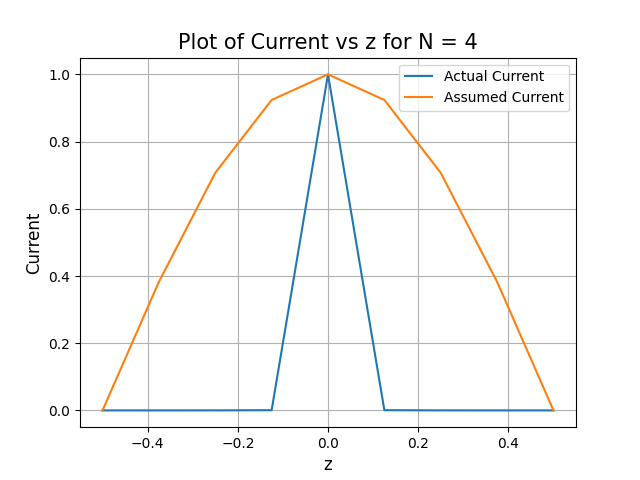
\includegraphics[scale = 0.8]{Figure_1.png}
    \label{fig:sample}
\end{figure}
The plot for N = 100 is:
\begin{figure}[H]
    \centering
    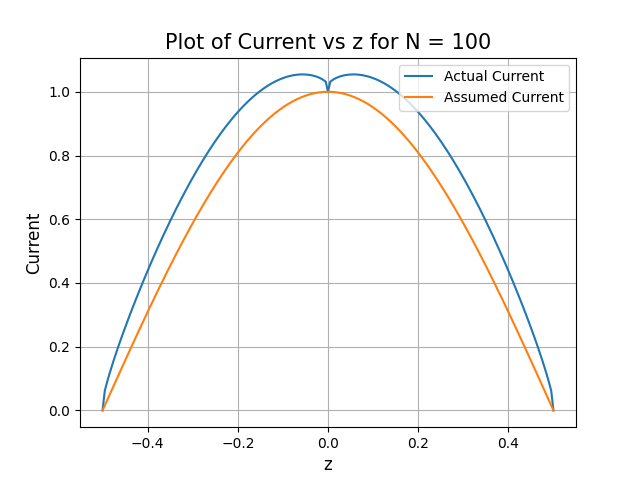
\includegraphics[scale = 0.8]{Figure_2.png}
    \label{fig:sample}
\end{figure}
From the above plots, we can see that the calculated $I$ is overshooting the assumed $I$ curve at all points. This is due to \textbf{error in integration} which leads to error in the value of current
\subsubsection{Output Vectors (For $N=4$)}
\begin{itemize}
    \item $ J :$
    $ 
    \begin{bmatrix}
        -3.30e-05+1.06e-05j \\ -9.55e-05+1.15e-05j \\ -6.48e-04+1.21e-05j \\ -6.48e-04+1.21e-05j \\ -9.55e-05+1.15e-05j \\ -3.30e-05+1.1e-05j
    \end{bmatrix}
    $ \\ \\
\item $ I : 
    \begin{bmatrix}
        0 \\ -3.30e-05+1.06e-05j \\ -9.55e-05+1.15e-05j \\ -6.48e-04+1.21e-05j \\  1 \\ -6.48e-04+1.21e-05j \\ -9.55e-05+1.15e-05j  \\ -3.30e-05+1.1e-05j \\ 0
    \end{bmatrix}
    $ \\ \\ 
\end{itemize}
\section{Conclusion}
\begin{itemize}
    \item Current profiles for wires in the antenna is calculated
    \item The assumed $I$ is a very close approximation to the assumed result
    \item The overshooting of calculated $I$ over the assumed $I$ is due to error in integration. Integration here was not done perfectly. Hence it leads to errors in $P,P_{B},Q,Q_{B}$ and hence error in $I$
\end{itemize}
\end{document}